\subsubsection*{15.23}


% \begin{wrapfigure}{r}{0.3\textwidth}
%   \begin{center}
%         \vspace{-20 mm}
%         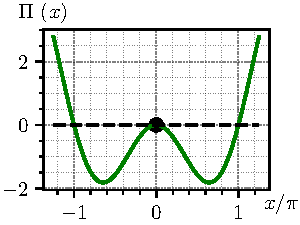
\includegraphics{figures/15_23.pdf}
%   \end{center}
%     \caption{График $\Pi(x) = -x\sin x$}
% \end{wrapfigure}

\begin{figure}
    \centering
    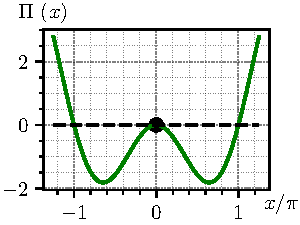
\includegraphics{figures/15_23.pdf}
    \caption{График $\Pi(x) = -x\sin x$}
\end{figure}


Начнём с того, что условие не корректно. 
Действительно, давайте посмотрим на близкие к $0$ положения равновесия системы с потенциалом $\Pi(x) = -x \sin x$. В точке $x=0$ существует неустойчивое положение равновесия, однако посмотрим на развитие системы из точки $\{-\pi-\delta, 0\}$, увидим, что на фазовой плоскости существует замкнутая орбита (сплюснутая в середине), содержащая $x=0$. Поэтому докажем, что при наличие устойчивого равновесия, существует замкнутая кривая на фазовой плоскости. 

Также хотелось бы что-то сказать при наличие замкнутой траектории о положении равновесия. Можно показать, что при отсутствие других положений равновесия в этой области положение равновесия будет устойчивым. Аналогично можно считать, что положение равновесия устойчиво только если для любой $U_\varepsilon$ окрестности существует замкнутая траектория вложенная в $U_\varepsilon$ и содержащая точку.

Так как сила $F = F(x)$ и $F(x)$ гладкая, то всегда можно ввести потенциал такой, что
\begin{equation*}
    -\frac{\partial \Pi(x)}{\partial x} = F(x) = \ddot{x}.
\end{equation*}
Также можно считать, что энергия системы сохраняется, то есть
\begin{equation*}
    E = \Pi(x) + \frac{1}{2} \dot{x}^2 = \const.
\end{equation*}

Пусть есть устойчивое положение равновесия $x^*$, тогда мы знаем, что
\begin{equation*}
    -\frac{\partial \Pi}{\partial x} (x^*) = 0, \hspace{0.5cm} \frac{\partial^2 \Pi}{\partial x^2} (x^*) > 0.
\end{equation*}
Тогда возьмём в в качетсве крайних точек нашей траектории $x_1 = x^* - \delta_1$ и в качетсве $x_2 = x^* + \delta_2$, где $\delta_i$ -- достаточно малая величина, чтобы $x' \notin U_\delta (x^*)$, $x' $ -- другое положение равновесия/точка перегиба потенциала. Выберем $\delta_1, \delta_2$ так, чтобы
\begin{equation*}
    \Pi(x^* - \delta_1) = \Pi(x^* + \delta_2).
\end{equation*}
Тогда поместив с 0 скоростью точку $x_1$ получим замкнутую орбиту $[x_1, \ x_2]$.

В другую сторону, пусть есть некоторая замкнутая орбита на $[x_1, \ x_2]$. Тогда верно, что
\begin{equation*}
    T(x_1) = T(x_2) = 0, \hspace{0.5cm} 
    -\frac{\partial \Pi}{\partial x} (x_1) > 0, \hspace{0.5cm} 
    -\frac{\partial \Pi}{\partial x} (x_2) < 0.
\end{equation*}
Тогда по непрерывности $\Pi(x)$ существует $x^*$ такой, что $\partial \Pi(x^*) / \partial x = 0$, при чём, так как это единственная точка перегиба потенциала в $[x_1, \ x_2]$, то $\partial^2 \Pi / \partial x (x^*) > 0$, Q. E. D.